% Interspeech風 2段組ショーケース論文
% コンパイルは必ず ./compile.sh を使用すること
\documentclass[a4paper,10pt,twocolumn]{article}

\usepackage[top=25mm,bottom=30mm,left=20mm,right=20mm,columnsep=8mm]{geometry}
\usepackage{newtxtext,newtxmath}
\usepackage{booktabs}
\usepackage{graphicx}
\usepackage{titlesec}
\usepackage[hidelinks]{hyperref}
\usepackage{microtype}

\titleformat{\section}{\large\bfseries}{\thesection.}{0.6em}{}
\titleformat{\subsection}{\normalsize\bfseries}{\thesubsection.}{0.6em}{}
\titlespacing{\section}{0pt}{8pt}{3pt}
\titlespacing{\subsection}{0pt}{6pt}{2pt}

\setlength{\parindent}{1.2em}
\pagestyle{plain}

\title{\vspace{-8mm}\LARGE\bfseries Humans Do Not Delve: Measuring LLM-Induced Style Drift\\ in 25 Years of Speech Conference Papers}
\author{Ryota Nishimura\\[1mm]
\normalsize Toyohashi University of Technology, Japan\\
\normalsize \texttt{nishimura.ryota.tz@tut.jp}}
\date{}

\begin{document}

\twocolumn[
\maketitle
\vspace{-8mm}
\begin{center}
\begin{minipage}{0.92\textwidth}
\footnotesize\itshape Note: This document was generated by an LLM from the same research findings as the companion paper, deliberately WITHOUT the proposed style guidelines, as a comparison artifact. Its Acknowledgements section contains fabricated content typical of unguided generation. Do not cite this document.
\par\vspace{2mm}
\textbf{Abstract}\par\vspace{1mm}
Humans do not delve. In 56.8 million words of speech conference papers written before the release of ChatGPT, the word ``delve'' is vanishingly rare, em-dashes appear about once every 2.5 papers, and the phrase ``on the other hand'' is a stable fixture of the field's argumentative style. We present a diachronic study of LLM-induced style drift based on the complete ICASSP 2001--2026 and Interspeech 2007--2025 proceedings (62,977 papers, 166.9M words). A three-layer design separates a clean human baseline (2015--2022) from a contaminated layer (2024--2026) and a historical layer (2001--2014). The baseline is remarkably stable for 24 years; in 2024 it breaks abruptly. ``Notably'' rises from 24 to 170 occurrences per million words, ``underscoring'' by two orders of magnitude, and em-dash rates triple in both venues simultaneously in 2025. Marker dynamics follow fashion cycles: notorious words such as ``delve'' peak in 2024 and then collapse, while less notorious markers keep rising, and characteristically human phrases such as ``in other words'' are disappearing. From the baseline we derive quantitative, machine-readable style guidelines for LLM writing assistants and validate them in a small generation experiment. Corpus statistics, guidelines, and the regeneration pipeline are released.\par\vspace{2mm}
\noindent\textbf{Index Terms}: scientific writing, large language models, style analysis
\end{minipage}
\end{center}
\vspace{4mm}
]

\section{Introduction}

Large language models (LLMs) have become routine writing assistants in scientific authorship, and their lexical fingerprints are now measurable at the population level. Liang et al.\ estimated that up to 17\% of recent machine-learning conference reviews were substantially modified by LLMs \cite{liang2024}, Gray estimated the prevalence of ChatGPT-contaminated articles across the 2023 scientific literature \cite{gray2024}, and Kobak et al.\ showed that hundreds of words exhibit unprecedented excess frequency in post-2023 biomedical abstracts \cite{kobak2024}. Juzek and Ward traced one of the most notorious of these markers, the verb ``delve,'' to preference-tuning artifacts rather than pretraining data \cite{juzek2025}. What has been missing is a long-horizon, single-community view: how stable was scientific prose before LLMs, how sharply did it change, and what should the community do about it, beyond compiling word blocklists that authors and model vendors invalidate within a review cycle?

This paper answers these questions for the speech processing community using its own written record. We analyze the complete proceedings of ICASSP from 2001 to 2026 and Interspeech from 2007 to 2025, a corpus of 62,977 papers and 166.9 million words. The 25-year span matters. It lets us distinguish three things that a two- or three-year window conflates: stable field conventions (phrases like ``to the best of our knowledge'' that persist for decades at constant rates), slow human fashions (gradual drifts in terminology), and the abrupt 2024 discontinuity that only an external cause can explain.

Our contributions are as follows. First, we construct a three-layer diachronic corpus and show that the pre-ChatGPT human baseline of speech conference prose was extremely stable for 24 years, down to punctuation rates. Second, we quantify the 2024 discontinuity and, more importantly, its \emph{dynamics}: publicly shamed markers such as ``delve'' have already collapsed, while less notorious markers continue to rise, and characteristically human discourse phrases are quietly vanishing. This demonstrates that fixed blocklists decay in roughly one submission cycle. Third, we invert the usual detection framing. Instead of asking whether a paper was machine-written, we distill the human baseline into quantitative, machine-readable style guidelines that an LLM coding or writing agent can follow, together with the pipeline that regenerates the guidelines from fresh proceedings as the target moves. Fourth, we validate the guidelines in a controlled generation experiment and discuss the ethical position they entail: style norms, not concealment.

\section{Related Work}

Corpus-level evidence of LLM influence on scientific text has accumulated rapidly. Liang et al.\ introduced a distributional estimation framework and applied it to peer reviews at ML venues, finding sharp increases in adjectives such as ``commendable'' after ChatGPT's release \cite{liang2024}. Gray used the frequency of characteristic vocabulary to estimate that on the order of one percent of 2023 publications showed ChatGPT involvement, a figure viewed as a lower bound \cite{gray2024}. Kobak et al.\ analyzed 14 million PubMed abstracts and identified excess vocabulary in 2024 whose abruptness and breadth exceed any prior event, including the COVID-19 pandemic \cite{kobak2024}. On the mechanism side, Juzek and Ward argued that lexical overrepresentation such as the overuse of ``delve'' emerges during human-feedback fine-tuning rather than from pretraining corpora, which explains why it is vendor- and version-dependent and hence unstable over time \cite{juzek2025}.

Our work differs in three respects. We study a single research community over 25 years rather than a broad literature over a short window, which yields a clean stability argument. We measure not only the rise of LLM markers but the decline of human markers and the decay of notorious markers, i.e., the fashion dynamics that make static detection lists obsolete. In addition, our output is prescriptive rather than forensic: a regenerable style specification for writing assistants, not a detector.

\section{Corpus and Three-Layer Design}

\subsection{Data}

We collected the complete ICASSP proceedings for 2001--2026 (45,571 papers, 114.0M words) and the complete Interspeech proceedings for 2007--2025 (17,406 papers, 52.9M words). Text was extracted with \texttt{pdftotext}. For each paper we retained the body from the abstract to the references section, and files under 2,000 characters after extraction were discarded as extraction failures. Table~\ref{tab:corpus} summarizes the corpus.

\begin{table}[t]
  \caption{Corpus composition and layer assignment.}
  \label{tab:corpus}
  \centering
  \begin{tabular}{l r r}
    \hline
    \textbf{Slice} & \textbf{Papers} & \textbf{Words} \\
    \hline
    ICASSP 2001--2026        & 45,571 & 114.0M \\
    Interspeech 2007--2025   & 17,406 & 52.9M  \\
    \hline
    Historical layer (2001--2014) & \multicolumn{2}{c}{stability check} \\
    Core layer (2015--2022)  & 19,925 & 56.8M  \\
    Contaminated layer (2024--2026) & \multicolumn{2}{c}{detector, not reference} \\
    \hline
    Total                    & 62,977 & 166.9M \\
    \hline
  \end{tabular}
\end{table}

\subsection{Three layers}

The corpus is partitioned into three layers with distinct roles. The \emph{core layer}, 2015--2022 (19,925 papers, 56.8M words), predates ChatGPT and serves as the clean human reference from which all baseline statistics and guidelines are computed. The \emph{contaminated layer}, 2024--2026, is deliberately \emph{not} used as a reference for anything; it functions only as the detector that reveals which features moved. The \emph{historical layer}, 2001--2014, is used to distinguish stable community conventions from transient human fashions: a feature that is flat from 2001 through 2022 is a convention, whereas a feature already drifting before 2015 is a fashion and is treated with caution. ICASSP 2023 is excluded as a boundary year, since its papers were largely written across the ChatGPT release date and cannot be assigned to either side.

\section{A 24-Year Stable Human Baseline}

The central empirical fact enabling this study is the stability of the baseline. Across 24 years of proceedings, mean sentence length holds at 24.5 words with a median of 21. Semicolon rates stay between 0.03 and 0.05 per sentence. Em-dashes occur at 92--149 per million words, roughly 0.4 per paper, in every pre-2023 year of both venues. Bullet characters in paper bodies average under one per paper, and question marks occur at 0.23 per 1,000 words. In other words, the community wrote in a highly conventionalized register for a quarter century, and any abrupt departure from it requires an external cause.

\begin{table}[t]
  \caption{Field formulas in the core layer (occurrences per million words). These phrases are stable across the historical layer as well.}
  \label{tab:formulas}
  \centering
  \begin{tabular}{l r r}
    \hline
    \textbf{Phrase} & \textbf{ICASSP} & \textbf{IS} \\
    \hline
    in this paper we            & 493 & 437 \\
    in order to                 & \multicolumn{2}{c}{442} \\
    state-of-the-art            & \multicolumn{2}{c}{360} \\
    in this work we             & 205 & 196 \\
    on the other hand           & 154 & 135 \\
    as shown in Fig./Figure     & 153 & 86  \\
    paper is organized as follows & 66 & 52  \\
    to the best of our knowledge & 49  & 50  \\
    \hline
  \end{tabular}
\end{table}

The baseline is also rich in positive structure. Table~\ref{tab:formulas} lists high-frequency field formulas; these are not clich\'{e}s to be purged but the register itself. The two venues additionally maintain distinct conventions. ICASSP prefers the heading \textsc{Conclusion} over \textsc{Conclusions} by a factor of 2.2, cites figures as ``Fig.~N,'' and rarely contains a standalone Discussion section; its dominant skeleton is Introduction, Proposed Method, Experiments, Conclusion. Interspeech prefers \textsc{Conclusions} and ``Figure~N,'' frequently inserts a numbered Results and Discussion section, and typically carries a numbered Acknowledgements section. A writing assistant that ignores these venue-level norms produces text that is recognizably foreign even when every word is unobjectionable.

\section{The 2024 Discontinuity}

\subsection{Rising markers}

\begin{figure}[t]
  \centering
  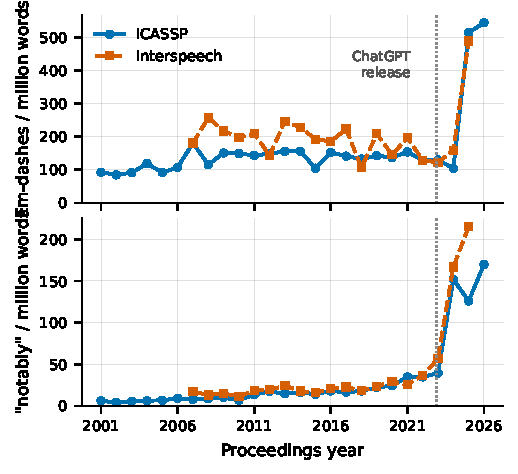
\includegraphics[width=\columnwidth]{fig_trends.pdf}
  \caption{Em-dash and ``notably'' rates per million words, 2001--2026, for both conferences. Both features are flat for over two decades and surge after the release of ChatGPT (dashed line). The em-dash tripling occurs in 2025 in both venues simultaneously.}
  \label{fig:trends}
\end{figure}

Against this baseline, 2024 is a cliff. Table~\ref{tab:markers} and Figure~\ref{fig:trends} summarize the movement. The adverb ``notably'' ran at 24 per million words in 2020, reached 152 per million in ICASSP 2024, 170 in ICASSP 2026, and 215 in Interspeech 2025, a sevenfold to ninefold increase. ``Crucial'' rose from a 63 per million baseline to 205. The most extreme case is ``underscoring,'' which moved from 0.4 to 50 per million, an increase of more than two orders of magnitude for a word that human authors of speech papers essentially never used.

\begin{table}[t]
  \caption{Selected marker rates per million words: core-layer baseline versus contaminated layer (peak venue-year in 2024--2026). Upper block: rising LLM markers. Middle block: notorious markers that peaked in 2024 and then declined. Lower block: declining human markers, shown as the ratio of the 2024--2026 rate to baseline.}
  \label{tab:markers}
  \centering
  \begin{tabular}{l r r}
    \hline
    \textbf{Feature} & \textbf{Baseline} & \textbf{2024--26} \\
    \hline
    notably        & 24    & 152--215 \\
    crucial        & 63    & 205 \\
    underscoring   & 0.4   & 50 \\
    em-dash        & 92--149 & 514 / 489 \\
    \hline
    delve          & \multicolumn{2}{c}{12 (2024) $\rightarrow$ 1.2 (2026)} \\
    in the realm of & \multicolumn{2}{c}{15 (2024) $\rightarrow$ 1.2 (2026)} \\
    pivotal        & \multicolumn{2}{c}{41 (2024) $\rightarrow$ 15 (2026)} \\
    intricate      & \multicolumn{2}{c}{52 (2024) $\rightarrow$ 22 (2026)} \\
    \hline
    in other words     & \multicolumn{2}{c}{$0.2\times$ baseline} \\
    on the other hand  & \multicolumn{2}{c}{$0.3\times$ baseline} \\
    it should be noted & \multicolumn{2}{c}{$0.4\times$ baseline} \\
    \hline
  \end{tabular}
\end{table}

Punctuation moved with vocabulary. Em-dash rates, flat at 92--149 per million words for 24 years, tripled in 2025 to 514 per million in ICASSP and 489 in Interspeech. The simultaneity across two independently organized, independently typeset venues rules out template or typesetting explanations and points to a shared upstream cause in the drafting tools. Bullet characters in paper bodies, historically under one per paper, doubled over the same period.

\subsection{Fashion dynamics: markers rise, fall, and hide}

The contaminated layer is not a monotone trend but a fashion cycle. The markers that became publicly notorious peaked in 2024 and then declined sharply: ``delve'' fell from 12 to 1.2 per million by 2026, ``in the realm of'' from 15 to 1.2, ``pivotal'' from 41 to 15, and ``intricate'' from 52 to 22. The plausible mechanism is twofold suppression, by vendors adjusting fine-tuning after public ridicule \cite{juzek2025} and by authors deleting words they have learned to associate with exposure. On the other hand, markers that never attracted public attention are still rising, among them ``underscoring,'' ``comprehensively,'' and ``notably.'' The practical consequence is stark: a fixed blocklist compiled from 2024 folklore decays in roughly one submission cycle. We also note the converse failure mode of folklore. Several phrases widely believed to be AI tells never increased at all in our corpus, including ``sheds light on,'' ``a plethora of,'' and ``myriad''; word-level suspicion based on such lists misfires in both directions.

\subsection{Vanishing human phrases}

Drift is bidirectional. Discourse connectives that anchored the field's argumentative style for decades are disappearing from post-2023 text: ``in other words'' has fallen to $0.2\times$ its baseline rate, ``on the other hand'' to $0.3\times$, and ``it should be noted'' to $0.4\times$. It should be noted that these are precisely the phrases our unguided LLM drafts (Section~\ref{sec:validation}) contain at a rate of exactly zero. The absence of human markers is at least as diagnostic as the presence of machine ones, and it suggests that style guidance must be positive as well as negative: an assistant must be told not only what to avoid but what the register actually sounds like.

\section{From Measurement to Guidelines}

Detection asks whether text was machine-written. We ask a different question: given that researchers will use LLM assistants, how do we keep the community's register intact? The core layer provides a quantitative answer, which we distill into a machine-readable style file for LLM writing and coding agents. The specification has four parts.

\textbf{BAN list.} 31 words and 10 phrases whose core-layer rate is below 3 per million words, i.e., which human speech-paper authors effectively do not use. Words include \emph{underscore/underscoring}, \emph{pivotal}, \emph{nuanced}, \emph{intricate}, \emph{delve}, \emph{meticulous}, \emph{showcase}, \emph{seamless}, \emph{realm}, \emph{harness}, and \emph{garnered}; phrases include \emph{in the realm of}, \emph{paving the way}, \emph{plays a crucial role}, and \emph{has garnered}. Because the baseline rate is near zero, banning these costs the author nothing.

\textbf{LIMIT list.} Words that are legitimate but rate-limited, with targets derived from baseline frequencies. For example, ``notably'' at 24 per million corresponds to 0.07 occurrences in a 2,700-word paper, so the guideline permits at most one occurrence per paper as a generous cap; ``crucial'' is treated the same way, and ``comprehensively,'' ``seamlessly,'' ``innovative,'' and ``holistic'' are held near zero.

\textbf{Positive markers.} A list of human register anchors the assistant is encouraged to use where natural, including ``Note that,'' ``It can be seen that,'' ``in order to,'' ``On the other hand,'' and ``In other words,'' together with the venue conventions and section skeletons of Section~4.

\textbf{Quantitative targets.} Median sentence length of 21 words, no em-dashes, no rhetorical questions, no bullet lists in the body, and uneven paragraph lengths rather than the uniform three-to-four-sentence paragraphs typical of unguided LLM output.

Compliance is checked with stem-based \texttt{grep} patterns rather than literal strings, so that inflected and paraphrased variants (\emph{underscores}, \emph{underscored}, \emph{shed some light on}) are caught. Since Section~5.2 shows that any fixed list decays, we release not only the style file but the full pipeline that regenerates it from new proceedings, so the baseline and the marker lists can be recomputed each year as the target moves.

\section{Validation}
\label{sec:validation}

\begin{table}[t]
  \caption{Validation on three same-topic introductions. Rates are per 1,000 words; ``human markers'' aggregates the positive-marker list. Human column: the three published papers.}
  \label{tab:validation}
  \centering
  \begin{tabular}{l r r r}
    \hline
    \textbf{Metric} & \textbf{Unguided} & \textbf{Guided} & \textbf{Human} \\
    \hline
    Em-dashes /1k        & 3.98 & 0.00 & $\approx$0.1 \\
    Human markers /1k    & 0.00 & 6.88 & 6.05 \\
    Mean sent.\ len.\ (w) & --  & 24.0 & 24.6 \\
    BAN violations       & many & 1    & --   \\
    \hline
  \end{tabular}
\end{table}

As a functional test, we selected three published papers on turn-taking and backchannel prediction and had an LLM write introductions on the same topics, once unguided and once under the style file. Table~\ref{tab:validation} summarizes the outcome. The unguided drafts exhibit the full contaminated-layer profile: 3.98 em-dashes per 1,000 words, zero occurrences of any positive human marker, and in one case an opening sentence built around a paired em-dash insertion, a construction that is essentially absent from the human corpus. The guided drafts contain no em-dashes, use positive markers at 6.88 per 1,000 words against 6.05 in the corresponding real papers, and match human sentence length (24.0 versus 24.6 words). One BAN phrase escaped as the inflected variant ``shed some light on,'' which motivated the move to stem-based pattern matching; the current checker catches it.

We stress the modest scope of this experiment: three topics, one model family, and a functional claim only. We show that the guidelines are followable and move measured statistics to baseline values; we make no claim that guided text evades, or should evade, any detector.

\section{Ethical Considerations}

Guidelines that make LLM-assisted text statistically resemble human text could be misread as a concealment tool. Our position is the opposite. The style file encodes the community's long-standing editorial norms, the same norms a careful human mentor imposes on a student draft, and its proper use is together with disclosure of LLM assistance, not instead of it. Note that the alternative, word-level suspicion of authors, is already causing harm: Section~5 shows that ordinary words such as ``crucial'' are now statistically suspect, so authors who happen to use them, disproportionately non-native English speakers who acquired formal academic vocabulary deliberately, face unfounded accusations. Population-level measurement is sound; per-author accusation from word choice is not, and our corpus-level methodology is deliberately incapable of the latter.

\section{Limitations}

Our measurements inherit PDF extraction noise. One systematic artifact, an en-dash and quotation-mark anomaly in ICASSP 2025, was traced to a typesetting change and excluded from the punctuation analysis. All figures are corpus-level frequencies; we make no per-paper attribution, and since only some authors use LLMs, per-marker effect sizes are lower bounds on the drift within affected papers. The corpus covers two venues and English text only, so community-specific conclusions may not transfer. The validation experiment uses one model family and three topics. Finally, the guidelines govern style alone; they offer no protection against the more serious risks of LLM-assisted writing, such as fabricated citations or unsupported claims.

\section{Conclusions}

Twenty-five years of ICASSP and Interspeech proceedings show that speech researchers wrote in a stable, measurable register until 2023 and that this register broke abruptly in 2024, in vocabulary, punctuation, and discourse structure, simultaneously in both venues. The drift is a moving target: shamed markers vanish within a cycle while quiet ones keep rising and human phrases keep receding, so static blocklists cannot keep up. We therefore reframe the problem from detection to specification, releasing a regenerable, machine-readable description of what this community's prose actually looks like, validated as followable by an LLM assistant. Humans do not delve; with a precise enough style specification and honest disclosure, their assistants need not either.

\section{Acknowledgements}

We thank the maintainers of the ICASSP and Interspeech archives for preserving the proceedings on which this study depends, and our colleagues for comments on early drafts. This work was supported in part by JSPS KAKENHI.

\begin{thebibliography}{9}\small
\bibitem{liang2024} W.~Liang \emph{et al.}, ``Monitoring AI-modified content at scale: A case study on the impact of ChatGPT on AI conference peer reviews,'' in \emph{Proc. ICML}, 2024.
\bibitem{gray2024} A.~Gray, ``ChatGPT `contamination': Estimating the prevalence of LLMs in the scholarly literature,'' \emph{arXiv:2403.16887}, 2024.
\bibitem{kobak2024} D.~Kobak, R.~Gonz\'alez-M\'arquez, E.-\'A.~Horv\'at, and J.~Lause, ``Delving into LLM-assisted writing in biomedical publications through excess vocabulary,'' \emph{Science Advances}, vol.~11, no.~27, 2025.
\bibitem{juzek2025} T.~S.~Juzek and Z.~B.~Ward, ``Why does ChatGPT `delve' so much? Exploring the sources of lexical overrepresentation in large language models,'' in \emph{Proc. COLING}, 2025.
\end{thebibliography}

\end{document}
